\documentclass[13pt]{article}
\usepackage[francais]{babel}
\usepackage[utf8]{inputenc}
\usepackage[T1]{fontenc}

\usepackage{verbatim}
\usepackage{amsthm}
\usepackage{amsmath,amssymb,amstext}
\usepackage{thmbox}
\usepackage{fancyhdr}
\usepackage{graphicx}
\usepackage{wrapfig}
\usepackage{url}


\newtheorem{bin}{ \textbf{Logique Binaire} }
\newtheorem{arit}{ \textbf{Arithmétique} }
\newtheorem{instr}
{ \textbf{Instructions actuellement prises en charges} }
\newtheorem{instrFutures}
{ \textbf{Instructions à venir} }

\newcommand{\cg}{[\kern-0.15em [}
\newcommand{\cd}{]\kern-0.15em ]}

\pagestyle{fancy}
\rhead{}

\title{Rapport du Projet de Système digital \no2}
\author{Belghiti Ismael, Desfontaines Damien, Geoffroy Guillaume, Maillard Kenji}
\date{\today}

\begin{document}
\renewcommand{\labelitemi}{$\triangleright$}
\maketitle

\section{Introduction}

Nous avons fini la création du simulateur de circuit et du langage
de description du circuit. Depuis le rapport $\no1$,
le langage a légèrement évolué grâce à des fonctionnalités supplémentaires
d'ordre pratique, comme le fait de pouvoir coder directement une certaine
suite binaire avec une syntaxe du type \$010011, la possibilité de
commenter le code source ou de le séparer en plusieurs fichiers. Nous
ne nous attarderons pas sur ces modifications mineures, bien qu'elles
enrichissent l'ergonomie du langage et permettent un développement plus serrein 
du microprocesseur

Ce rapport décrit donc l'étape suivante, c'est-à-dire le dessin du
microprocesseur, ses caractéristiques techniques ainsi que son utilisation.

\section{Inspiration et dessin du microprocesseur}

Pour le dessin du microprocesseur, nous nous sommes inspirés des schémas
de fonctionnement MIPS présents dans l'ouvrage \textit{Computer Organization and Design}.
Nous donc reprenons ici le schéma global de fonctionnement, tiré de
cet ouvrage :

\begin{figure}[!h]
\centering
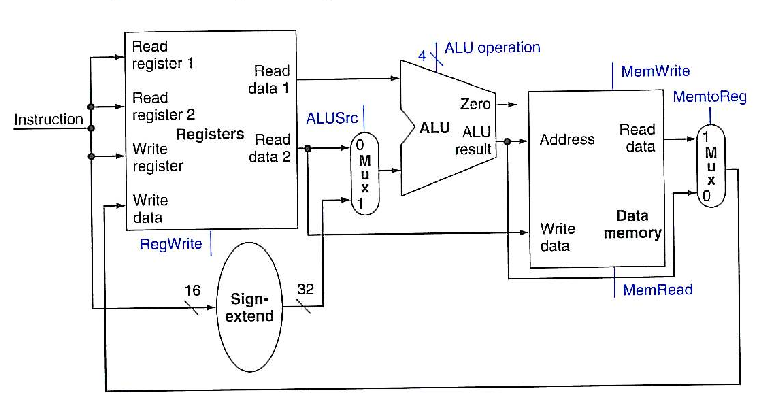
\includegraphics[width=9cm,height=50mm]{ArchitectureMipsSimple.png}
\caption{Architecture MIPS}
\label{Architecture MIPS}
\end{figure}


Décrivons les différents blocs présents sur ce schéma qu'il a fallu
implémenter. 

\subsection{ALU}


\paragraph*{Principe :}

L'ALU que nous avons réalisé prend en entrée deux entiers sur 32 bits ainsi 
qu'un code sur 4 bits décrivant l'opération à effectuer. Il renvoie
alors un résultat sur 32 bits. Il s'agit d'un bloc
purement combinatoire : rien n'est stocké dans l'ALU, qui ne contient
donc aucun registre et effectue toutes les opérations en un seul cycle.


\paragraph*{Opérations implémentées :}

Les opérations implémentées sont les opérations arithmétiques et logiques
classiques : + , - , {*} , And, Or, Xor, Nand, Nor ... (la division n'est
pour l'heure pas incluse). Le fichier Alu.rock présente ce bloc, les
commentaires à la fin du fichier devraient être suffisants pour pouvoir
lancer quelques tests.\\


Voici la liste complète des opérations définies ainsi que leurs codes 4 bits associés :\\


\begin{bin}


\begin{itemize}
   \item Et   : 0000
   \item Ou   : 1000
   \item Xor  : 0100
   \item Nand : 1100
   \item Nor  : 0010 
\end{itemize}

\end{bin}

\begin{arit}

\begin{itemize}
   \item Addition       : 1010
   \item Soustraction   : 0110
   \item Multiplication : 1110
   \item Egalité        : 0001
   \item Différence     : 1001
   \item Infériorité stricte : 0101 
   \item Supériorité stricte : 1101
   \item Infériorité large   : 0011
   \item Supériorité large   : 1011 
\end{itemize}

\end{arit}

Dans notre code, il s'agit du bloc 
\textit{Alu<m>(a[m], b[m], sel[4])}, $m$ étant
une variable permettant de définir le nombre de bits
sur lequel on travaille (utile pour faire des tests).

\paragraph*{Comment ça marche :}

Chaque opération de l'ALU est codée séparément. Puis, à la lecture
de deux entiers, toutes les opérations possibles sont exécutées simultanément,
et un filtre sélectionne le résultat voulu. Tout fonctionne en un
seul cycle, et les circuits correspondant aux diverses opérations
ont tous été codés récursivement.

\subsection{Registres}

Le gestionnaire de registres contient 32 registres de 32 bits 
chacun. Il prend en entrée trois arguments : un booléen indiquant
si l'on est en mode écriture ou en mode lecture, l'adresse du registre
concerné, et la valeur sur 32 bits à éventuellement écrire. 

La sortie est alors la valeur du registre à lire si l'on est
en mode lecture, l'ancienne valeur du registre réaffecté si l'on
est en mode écriture (cette dernière valeur est généralement 
ignorée).

On remarquera
que l'on ne peut accéder qu'à un seul registre 
à la fois avec ce modèle. Nous envisageons la possibilité
de passer à un modèle avec plus d'accès simultanés
ce qui pourrait permettre d'alléger le controleur et travailler
sur moins de cycles pour chaque instruction. 
Cette possibilité sera discutée durant la séance du 5 janvier.\\
 
Le bloc générique actuel est
\textit{Gestionnaire<n,m>(modeEcriture, sel[5], val[m])}.
$n$ désigne le nombre de registres et $m$ le nombre de bits
de chaque registre
($n$ et $m$ sont tous deux fixés à 32 par la suite)

\subsection{Instruction Memory et Data Memory}

Pour l'instant il n'y a pas de Data Memory, ce bloc
sera implémenté bientôt à l'aide de devices. 
Le bloc Instruction Memory est actuellement utilisé
pour tester différents petits programmes, sa structure 
sera donc amenée à changer lorsque l'on voudra exécuter
le programme de l'horloge digitale.

\subsection{Controleur}

Le bloc de contrôle, présent dans notre projet sous le nom 
de ``Controleur''
a dans notre projet non 
seulement le rôle du bloc ``Control''
de l'architecture standart MIPS 
mais c'est aussi lui qui s'occupe
de la synchronisation entre 
les différents cycles parcourus pour une
instruction donnée (Tous les autres blocs
sont donc positionnés en étoile par rapport 
à lui). Cette synchronisation
est obtenue et sécurisée par l'utilisation de filtres
temporels gérant les trafics d'informations entre les
différents blocs.
Actuellement, toutes les instructions sont traitées en
3 cycles. Ce modèle pourra changer s'il on change
de type de gestionnaire de registres. \\

Ce Controleur agit différemment selon le format de 
l'instruction à effectuer, il contient donc plusieurs
décodeurs : un pour le \textit{R-format}, un pour le 
\textit{I-format},
un pour le \textit{J-format} et un pour les instructions
de type $branch$ qui sont techniquement en 
\textit{I-format} mais que
nous avons préféré traiter à part pour des raisons de
simplicité.\\

Dans notre code, le bloc correspondant est :
\textit{Controleur <b> (instr[32], alu[32], 
gestReg[32], pc[b])}, $b$, le nombre de bits
d'adressage des instructions, étant en paramètre
pour faciliter certains tests. Dans la suite, $b$ est
fixé à 26. 


\subsection{Instructions prises en charge}

Voici la liste des instructions actuellement prises en 
charges : 

\begin{instr}

\textbf{R-format}
\begin{itemize}
  \item and, funct : 000000
  \item or,  funct : 100000
  \item xor, funct : 010000 
  \item nor, funct : 001000
  \item add, funct : 101000
  \item sub, funct : 011000
  \item mult,funct : 111000
\end{itemize}

\textbf{I-format}
\begin{itemize}
  \item andi, opcode : 000011
  \item ori,  opcode : 100011
  \item xori, opcode : 010011 
  \item nori, opcode : 001011
  \item addi, opcode : 101011
  \item subi, opcode : 011011
  \item multi,opcode : 111011
\end{itemize}

\textbf{J-format}
\begin{itemize}
  \item jump, opcode : 111101
\end{itemize}

\textbf{branch-format}
\begin{itemize}
  \item beq, opcode : 111110
\end{itemize}

\end{instr}

\textit{}\\

On remarquera que les codes \textit{funct} des instructions
correspondant à un \textit{R-format} ainsi que les opcodes
des opérations en \textit{I-format} contiennent les codes
4 bits des opérations associées (voir section sur l'ALU),
ceci permet une implémentation simple. De même, 
on prend ici la convention dans laquelle on peut connaître
le format d'une instruction à travers les deux derniers bits
de son opcode : $00$ pour un \textit{R-format}, $11$ pour un 
\textit{I-format}, $01$ pour un \textit{J-format} et $10$ pour 
les instructions de type $branch$.\\

D'autres instructions sont prévues :

\begin{instrFutures}
\begin{itemize}
\item   bne
\item   jal
\item   jr
\item   lb
\item   lh
\item   lw
\item   sw
\item   sh
\item   sb
\item   lui
\item   mflo
\item   mfhi
\item   slt
\item   slt
\item   sll
\item   srl
\item   sra
\end{itemize}
\end{instrFutures}

\section{Prise en main}

En repartant des conventions précédentes
on peut par exemple construire l'instruction en 
\textit{R-format} suivante : \\
opcode : 000000 ; rs : 10000 ; rt : 01000 ; 
rd : 01000; shift : 00000; funct : 111000\\
qui s'écrit également :
00000010000010000100000000111000
et qui correspond à multiplier les registres d'adresses 10000
et 01000 et mettre le résultat dans le registre d'adresse
01000.\\

Pour écrire un programme, il suffit alors d'écrire une suite
d'instructions concaténées. Dans le fichier micro.rock, le
bloc créé est fait pour recevoir 8 instructions 
(sur 32 bits chacune).
S'il on souhaite utiliser moins d'instructions, il suffit de
rajouter des instructions inutiles à la suite du programme.
Pour augmenter le nombre d'instructions utilisables, il
suffit de modifier la dernière ligne du fichier rock en
changeant le 8 par un nombre plus grand. \\


Plusieurs programmes sont donnés 
pour tester le microprocesseur.
On les trouve décrits dans le dossier \textit{testMicro}.
Les fichiers \textit{fibo.prog} (calcul des termes de la suite
de Fibonacci), \textit{facto.prog} (calcul des factorielles), et 
\textit{beq.prog} (une utilisation simple d'un \textit{branch}) 
sont décrits respectivement dans \textit{fibo.exp}, \textit{facto.exp}
et \textit{beq.exp}.\\

Voici par exemple le code de fibo.prog :\\
\textit{}\\
$10101100000000001000000000000000$\\
$10101110000100001000000000000000$\\
$00000010000000000100000000101000$\\
$10101110000000000000000000000000$\\
$10101101000100000000000000000000$\\
$11110101000000000000000000000000$\\
$00000000000000000000000000000000$\\
$00000000000000000000000000000000$\\


Pour faire executer ce programme par le microprocesseur, 
il faut compiler le fichier micro.rock
puis, en supposant l'exécutable obtenu et le fichier 
fibo.prog dans le dossier courant, executer la ligne de 
commandes : \\
./micro -s 50 < fibo.prog\\
\textit{}\\
On obtient alors les sorties de l'Alu à chaque cycle 
(50 désigne ici le nombre de cycles désiré).

\section{Conclusion et travail à venir}

Le langage de description élaboré nous a permis 
de décrire de façon adaptée
une grande partie du microprocesseur qui 
est à ce jour capable d'exécuter de petits programmes.
Le travail restant consiste principalement élargir 
le set d'instructions du microprocesseur, éventuellement 
restructurer certaines parties de celui-ci, l'optimiser à l'aide 
de 
\textit{devices} et d'\textit{enables} déjà disponibles mais
non encore utilisés, et également implémenter une mémoire.
L'élaboration de la montre digitale pourra se faire en 
parallèle et l'afficheur 7 segments est déjà implémenté.

\end{document}






